\documentclass[a4paper,11pt]{article}

\usepackage[spanish]{babel}
\usepackage[utf8]{inputenc}

\usepackage{amsmath}
\usepackage{siunitx}

\usepackage{graphicx}
\usepackage{float}
\usepackage[font=small,labelfont=bf]{caption}
\usepackage[colorlinks=true]{hyperref}

\usepackage{booktabs}
\usepackage{multirow}

\title{Caracterización de componentes electrónicos utilizando una placa de audio}
\date{\today}
\author{Micaela Toscani, Axel Lacapmesure y Guillermo Brinatti}

\begin{document}
\maketitle



\section{Introducción}

\section{Desarrollo de la aplicación de adquisición}
\label{sec:software}

	El control de la placa de adquisición fue llevado a cabo a partir de programar una biblioteca propia en lenguaje Python \cite{repo}. La misma incluyó funciones orientadas al usuario final destinadas a utilizar el dispositivo para la adquisición de datos y la generación de trenes de pulsos configurables, tanto en los modos de disparo único como de ejecución continua. Para ello empleamos la biblioteca \emph{\href{https://nidaqmx-python.readthedocs.io}{nidaqmx}} propia del fabricante de la placa de adquisición \cite{nidaqmx}, y que provee una API para la configuración del dispositivo y para su comunicación a través de los controladores del mismo.
	
	Las funciones de usuario final se encargaron de la configuración de los canales de entrada analógicos y salidas de contadores, de la adquisición de una muestra finita de largo arbitrario, y de la adquisición continua de datos en simultáneo con la generación de pulsos de anchos variables. En la figura \ref{fig:flujo_software} se muestra un diagrama de flujo de una ejecución típica para la adquisición y generación de pulsos en modo continuo. Asimismo la biblioteca incluyó los elementos necesarios para la implementación del lazo de control que se discutirá en la sección \ref{sec:control_temperatura}, a saber, las estructuras que manejan la entrada de datos de sensado, que calculan la señal de error y que generan la señal de hacia el actuador.
	
	El la adquisición de lectura y escritura se basa en un bucle que en cada iteración adquiere una ventana de datos con un número fijo de muestras, las procesa y por último escribe la configuración de los pulsos de salida, esto es, su frecuencia de repetición y su ancho. Para el funcionamiento de este esquema se asume que el tiempo de ejecución de las instrucciones dentro de cada iteración es menor al tiempo que demora la adquisición de las muestras, de manera que no se produzcan sobrecargas en el \emph{buffer} de la placa de adquisición. Bajo el modo de disparo único, las sucesivas ventanas temporales se concatenan en una variable de salida preinicializada, y el bucle finaliza cuando el número de muestras adquiridas alcanza el número total configurado. Bajo el modo de ejecucuón continua, las ventanas temporales se sobreescriben, y el bucle finaliza cuando el usuario interrumpe manualmente la ejecución del programa con el comando de teclado. En ambos casos, la finalización del bucle desencadena la etapa de cierre de comunicaciones y, eventualmente, el gráfico y guardado de los datos.
	
	\begin{figure}[!h] 
        \centering
        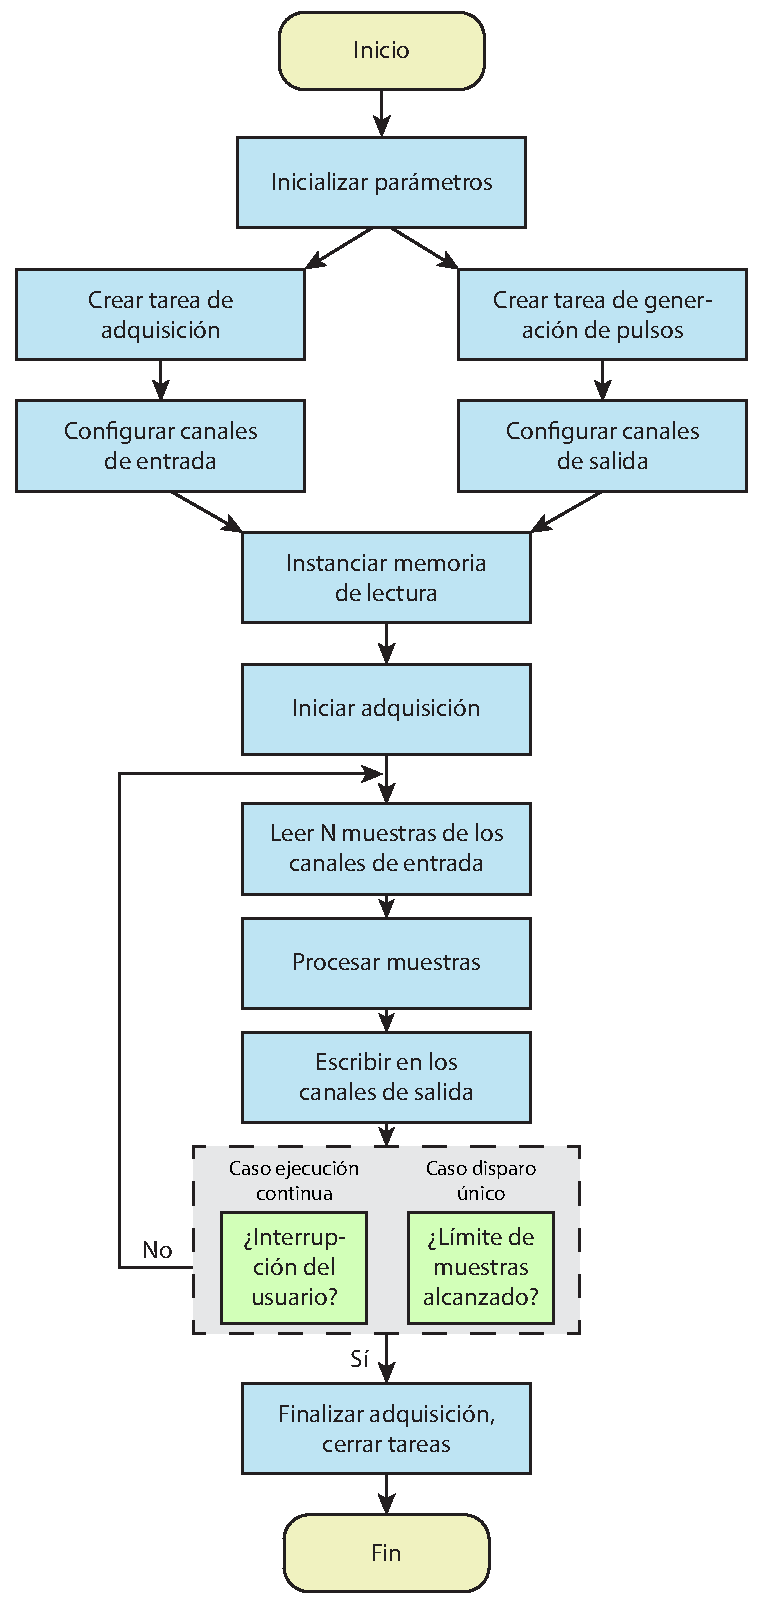
\includegraphics[height=.95\textheight]{flujo_software.pdf}
        \caption{Diagrama de flujo para la aplicación de adquisición y generación de pulsos en modo de disparo único y ejecución continua.}
        \label{fig:flujo_software}
 
    \end{figure}
	

\section{Caracterización de la placa de adquisición}

\section{Control de temperatura}
\label{sec:control_temperatura}

\subsection{Implementación de un lazo de control}

\subsection{Implementación de un lazo de control PID}




\clearpage

\begin{thebibliography}{99}

	\bibitem{repo} Repositorio en GitHub de la biblioteca propia utilizada en el trabajo, \href{https://github.com/fotonicaOrg/daq}{URL: https://github.com/fotonicaOrg/daq}, actualizado el 7/11/2018. La biblioteca está programada en el archivo \emph{daq.py}.
	\bibitem{nidaqmx} Documentación de la biblioteca nidaqmx, \href{https://nidaqmx-python.readthedocs.io}{URL: https://nidaqmx-python.readthedocs.io}, accedido el 7/11/2018.


\end{thebibliography}



\end{document}
